\documentclass[tikz,border=6pt]{standalone}
\usepackage{amsmath}
\usepackage{xcolor}
\usetikzlibrary{arrows.meta}

\definecolor{axisgray}{HTML}{333333}
\definecolor{lineblue}{HTML}{4A90D9}
\definecolor{linered}{HTML}{E74C3C}

\begin{document}
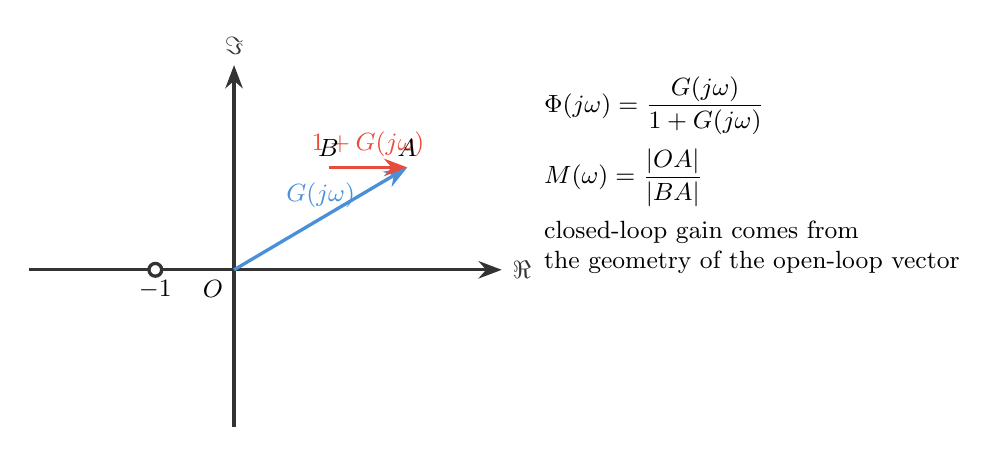
\begin{tikzpicture}[>=Stealth, line width=1.2pt, font=\small]
  \draw[axisgray, ->] (-2.6,0) -- (3.4,0) node[right] {$\Re$};
  \draw[axisgray, ->] (0,-2.0) -- (0,2.6) node[above] {$\Im$};
  \coordinate (O) at (0,0);
  \coordinate (A) at (2.2,1.3);
  \coordinate (B) at (1.2,1.3);
  \draw[lineblue, ->] (O) -- (A) node[midway, above] {$G(j\omega)$};
  \draw[linered, ->] (B) -- (A) node[midway, above] {$1+G(j\omega)$};
  \filldraw[fill=white, draw=axisgray] (-1,0) circle (2.3pt);
  \node[below] at (-1,0) {$-1$};
  \node[below left] at (O) {$O$};
  \node[above] at (A) {$A$};
  \node[above] at (B) {$B$};
  \node[align=left, anchor=west] at (3.8,1.2) {
    $\displaystyle \Phi(j\omega)=\frac{G(j\omega)}{1+G(j\omega)}$\\[4pt]
    $\displaystyle M(\omega)=\frac{|OA|}{|BA|}$\\[4pt]
    closed-loop gain comes from\\
    the geometry of the open-loop vector
  };
\end{tikzpicture}
\end{document}
